\documentclass[ignorenonframetext, professionalfonts, hyperref={pdftex, unicode}]{beamer}

\usetheme{Copenhagen}
\usecolortheme{wolverine}

%Packages to be included
%\usepackage{graphicx}

\usepackage[russian]{babel}
\usepackage[utf8]{inputenc}
\usepackage[T1]{fontenc}

%%\usepackage[orientation=landscape, size=custom, width=16, height=9.75, scale=0.5]{beamerposter}

\usepackage{textcomp}

\usepackage{beamerthemesplit}

\usepackage{ulem}

\usepackage{verbatim}

\usepackage{ucs}


\usepackage{listings}
\lstloadlanguages{bash}

\lstset{escapechar=`,
	extendedchars=false,
	language=sh,
	frame=single,
	tabsize=2, 
	columns=fullflexible, 
%	basicstyle=\scriptsize,
	keywordstyle=\color{blue}, 
	commentstyle=\itshape\color{brown},
%	identifierstyle=\ttfamily, 
	stringstyle=\mdseries\color{green}, 
	showstringspaces=false, 
	numbers=left, 
	numberstyle=\tiny, 
	breaklines=true, 
	inputencoding=utf8,
	keepspaces=true,
	morekeywords={u\_short, u\_char, u\_long, in\_addr}
	}

\definecolor{darkgreen}{cmyk}{0.7, 0, 1, 0.5}

\lstdefinelanguage{diff}
{
    morekeywords={+, -},
    sensitive=false,
    morecomment=[l]{//},
    morecomment=[s]{/*}{*/},
    morecomment=[l][\color{darkgreen}]{+},
    morecomment=[l][\color{red}]{-},
    morestring=[b]",
}

\author[Epam]{{\bf Epam}\\Low Level Programming Department}

%\institution[EPAM]{EPAM}
%\logo{\includegraphics[width=1cm]{logo.png}}


\title{Сеть в ОС Linux\\Продолжение}


%%%%%%%%%%%%%%%%%%%%%%%%%%%%%%%%%%%%%%%%%%%%%%%%%
%%%%%%%%%% Begin Document  %%%%%%%%%%%%%%%%%%%%%%
%%%%%%%%%%%%%%%%%%%%%%%%%%%%%%%%%%%%%%%%%%%%%%%%%




\begin{document}

\begin{frame}
	\frametitle{}
	\titlepage
	\vspace{-0.5cm}
	\begin{center}
	%\frontpagelogo
	\end{center}
\end{frame}


%%%%%%%%%%%%%%%%%%%%%%%%%%%%%%%%%%%%%%%%%   
%%%%%%%%%% Content starts here %%%%%%%%%%
%%%%%%%%%%%%%%%%%%%%%%%%%%%%%%%%%%%%%%%%%

\section{Network namespaces}
\mode<all>{\begin{frame}[fragile]{netns}
    \begin{block}{Network namespace}
		Изолированное сетевое пространство для процесса или группы процессов,
        которое позволяет использовать отдельные:

        \begin{itemize}
            \item сетевые устройства
            \item таблицу маршрутизации
            \item правила файерволла
            \item arp-таблицу
        \end{itemize}
    \end{block}
\end{frame}

\begin{frame}[fragile]{ip netns}
    \begin{block}{Управление netns}
        \begin{itemize}
            \item Список -- {\tt ip netns list}
            \item Создать -- {\tt ip netns add <name>}
            \item Удалить -- {\tt ip netns add <name>}
        \end{itemize}
    \end{block}

    \begin{block}{Процессы и netns}
        \begin{itemize}
            \item Запуск процесса -- {\tt ip netns exec <name> <programm>}
            \item Список процессов -- {\tt ip netns pids <name> }
            \item Определение NS для процесса -- \\
                {\tt ip netns identify <PID>}
        \end{itemize}
    \end{block}
\end{frame}

\begin{frame}[fragile]{Упражнение}

    \begin{block}{Соединяем 2 netcat}
        \begin{enumerate}
            \item Создать netns 'A'
            \item Запустить {\tt bash} в netns 'A'
            \item Проверить список доступных интерфейсов
            \item Узнать в каком netns находится текущий шелл
            \item Запустить в netns 'A' сервер:\\
                {\tt netcat -l 80}
            \item Поробовать подключиться клиентом:
                {\tt netcat 127.0.0.1 80}
            \item Попробовать предыдущий пункт в netns 'A'
            \item Посмотреть сетевой статус клиента и сервера\\
                (Hint: {\tt netstat})
            \item Получить список PID программ, находящихся в netns 'A'
        \end{enumerate}
    \end{block}

\end{frame}

\begin{frame}[fragile]{Интерфейсы в netns}
    \begin{itemize}
        \item Переместить интерфейс в netns:\\
            {\tt ip link set dev <interface> netns <namespace>}\\
            {\tt ip link set dev <interface> netns <PID>}
        \item Соединение 2 network namespaces:
            \begin{enumerate}
                \item Создать {\tt veth} пару
                \item Переместить один из интерфейсов в нужный netns
            \end{enumerate}
    \end{itemize}
\end{frame}

\begin{frame}[fragile]{Упражнение}
    \begin{block}{''Независимая сеть''}
        \begin{enumerate}
            \item Создать дополнительный интерфейс {\tt ethA0} типа {\tt macvlan} на базе {\tt eth0}
            \item Переместить интерфейс {\tt ethA0} в netns 'A'
            \item Назначить интерфейсу {\tt ethA0} адрес из подсети {\tt 192.168.254.0/24}
            \item Проверить доступность соседа с помощью {\tt ping} 
            \item Запустить сервер {\tt netcat} в netns 'A'
            \item Подключиться клиентом {\tt netcat} к соседу
        \end{enumerate}
    \end{block}
\end{frame}

\begin{frame}[fragile]{Упражнение}
    \begin{block}{Внутренняя сеть}
        \begin{enumerate}
            \item Создать netns 'B'
            \item Создать пару {\tt veth} интерфейсов: {\tt vethA} и {\tt vethB}
            \item Переместить {\tt vethA} в netns 'A' и {\tt vethB} в netns 'B'
            \item Назначить интерфейсам адреса из одного диапазона (192.168.0.0/24)
            \item Узнать в каком netns находится текущий шелл
            \item Запустить в netns 'A' сервер:\\
                {\tt netcat -l 80}
            \item Запустить клиента {\tt netcat} в netns 'B'
        \end{enumerate}
    \end{block}
\end{frame}

\begin{frame}[fragile]{Упражнение}
    \begin{block}{Анализ трафика}
        \begin{enumerate}
            \item Запустить {\tt ping} адреса {\tt vethB} в netns 'A'
            \item Запустить {\tt tcpdump} на интерфейсе {\tt vethA}
            \item Ограничить трафик протоколом {\tt ICMP}:\\
                {\tt tcpdump -n icmp}
                \begin{itemize}
                    \item Использовать ключи {\tt -t}, {\tt -tt}, {\tt -ttt}
                \end{itemize}
            \item Ограничить трафик IP адресом {\tt vethB}:\\
                {\tt tcpdump -n host <IP>}
            \item Ограничить трафик IP адресом {\tt vethB} и портом сервера:\\
                {\tt tcpdump -n host <IP> and port <port>}
            \item Записать дамп соединения {\tt netcat} клиент-сервер.\\
                Добавить ключ "-w <имя\_файла>".
            \item "Проиграть" дамп соединения:\\
                Добавить ключ "-r <имя\_файла>".
        \end{enumerate}
     \end{block}
\end{frame}

\begin{frame}[fragile]{Упражнение}
    \begin{block}{''Визуализация'' с wireshark}
        \begin{itemize}
            \item Проанализировать записанную сессию с помощью {\tt wireshark}:\\
                {\tt wireshark <имя\_файла>}
        \end{itemize}
     \end{block}
\end{frame}

}

\section{Маршрутизация}
\mode<all>{\begin{frame}{Маршрутизация}
	\begin{itemize}
		\item netstat -r
		\item route
		\item ip route show
	\end{itemize}

	\begin{block}{Разрешить маршрутизацию на хосте}
		{\tt echo 1 > /proc/sys/net/ipv4/ip\_forward}
	\end{block}
\end{frame}


}

\section{iptables}
\mode<all>{\begin{frame}{Iptables}

	\center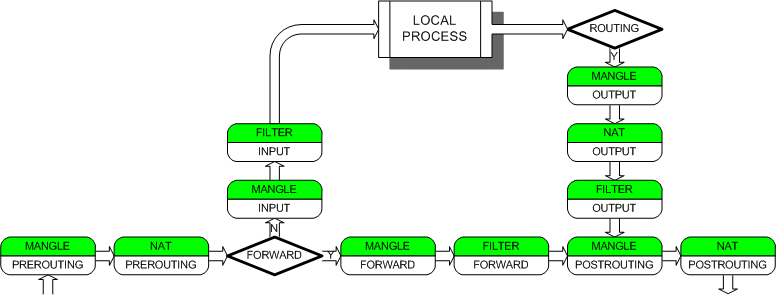
\includegraphics[height=0.4\textheight]{../../slides/networking/06-iptables.png}

	\begin{itemize}
	\begin{columns}
		\column{0.3\textwidth}
			\item[ ] {\bf iptables -L -t <table>}
				\bigskip

			\item filter -- файерволл
				\begin{itemize}
					\item INPUT
					\item FORWARD
					\item OUTPUT
				\end{itemize}
		\column{0.3\textwidth}
			\item nat -- преобразования адресов
				\begin{itemize}
					\item PREROUTING
					\item INPUT
					\item OUTPUT
					\item POSTROUTING
				\end{itemize}
		\column{0.3\textwidth}
			\item mangle -- специальные  изменения  пакетов (TOS, TTL, MARK)
				\begin{itemize}
					\item PREROUTING
					\item INPUT
					\item FORWARD
					\item OUTPUT
					\item POSTROUTING
				\end{itemize}
		\end{columns}
	\end{itemize}

\end{frame}


}

%%\mode<all>{\begin{frame}{Практика: создание тестовой среды}

	\center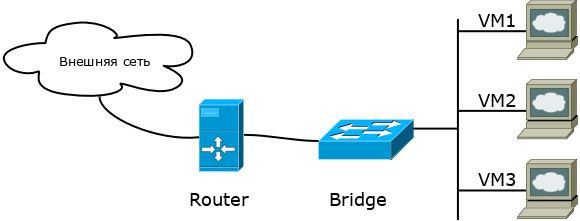
\includegraphics[height=0.4\textheight]{../../slides/networking/net-practice.png}


	\begin{block}{Задача}
		Запустить 3 идентичные виртуальные машины.\\
		Каждой машине назначить адрес из отдельного IP диапазона.\\
		Организовать сетевую ''видимость'' между виртуальными машинами, а также хостом.		
	\end{block}

\end{frame}



\begin{frame}
	\frametitle{Подготовка дисковой подсистемы}
			\begin{itemize}
				\item Создать пустой файл размером в 1.5 GB и отобразить на устройство
					/dev/loop ({\tt dd, losetup})
				\item Создать группу томов на базе этого устройства ({\tt pvcreate, vgcreate})
				\item Выделить 1 GB под логический диск ({\tt lvcreate})
				%\item Скопировать образ виртуального диска в полученный логический том ({\tt dd})
				%\item Создать снимок логического тома на 100MB ({\tt lvcreate}) для каждой виртуальной машины.
			\end{itemize}
\end{frame}

\begin{frame}[fragile]{Установка системы}
        \begin{itemize}
			\item Установить centos-minimal на  машину из iso файла.
            \item Создать два снимка логического тома виртуальной машины
			\item Убедиться в наличии tap интерфейсов
		\end{itemize}

\end{frame}

\begin{frame}[fragile]{Пример запуска kvm}
		\begin{itemize}
          \item {\tt modprobe kvm-intel} {\small Включаем модуль поддержки виртуализации в ядре} 
          \item {\tt modprobe tun}  {\small Включаем поддержку tun, tap виртуальных сетевых интерфейсов}
          \item 
            \begin{lstlisting}[language=bash,basicstyle=\tiny] 
kvm -enable-kvm -cdrom centos-minimal.iso -hda /dev/loop0 -m 512M   \
    -boot order=cd -serial stdio -net nic,model=rtl8139 -net tap,ifname=tap0 
            \end{lstlisting}
              \begin{enumerate}
                \item[{\tt -enable-kvm}] Включает ядерную поддержку виртуализации
                \item[{\tt -cdrom}] Устройство или disk image, cdrom виртуальной машины
                \item[{\tt -hda}] Устройство или disk image, представляет жесткий диск VM
                \item[{\tt -serial}] Перенаправление com порта (консоль ядра)
                \item[{\tt -net nic}] Условная модель сетевой карточки
                \item[{\tt -net tap}] TAP интерфейс, на который будет приходить сеть из VM
                \item[{\tt -boot order}] cd (вначале cdrom (с), потом диск (d))
                \item[{\tt -m}] Объем памяти для VM
              \end{enumerate}
        \end{itemize}
\end{frame}        


\begin{frame}
	\frametitle{Настройка сети на хосте}
			\begin{itemize}
				\item Создать мост {\tt brctl} и назначить ему адреса из соответствующих диапазонов {\tt ifconfig/ip}
				\item Поднять виртуальные интерфейсы {\tt ifconfig/ip}
				\item Добавить виртуальные интерфейсы к мосту {\tt brctl}
			\end{itemize}
\end{frame}


\begin{frame}
	\frametitle{Настройка сети на виртуальных машинах}
			\begin{itemize}
				\item Назначить адрес устройству eth0 {\tt ifconfig/ip}
				\item Добавить адрес маршрутизатора по умолчанию {\tt route/ip}
				\item Проверить доступность виртуальных машин и хоста {\tt ping/nmap}
			\end{itemize}
\end{frame}

\begin{frame}
	\frametitle{Настройка роутинга и NAT}
			\begin{itemize}
				\item Разрешить форвардинг на хосте
				\item Настроить NAT на хосте ({\tt iptables},  правило {\tt MASQUERADE})
				\item Проверить доступность хостов из ''внешней'' сети {\tt ping/nmap}
			\end{itemize}
\end{frame}


}

\mode<all>\begin{frame}[fragile]{Вопросы?}
    \setcounter{tocdepth}{2}
    \tableofcontents

    \bigskip

    \hrulefill
    \begin{columns}
    \column{0.7\textwidth}
            \center{Материалы:}
            \url{https://yadi.sk/d/Ixp8kHfl3MipCq}
    \column{0.2\textwidth}
        \begin{center}
            
\includegraphics[width=0.7\textwidth]{url-qr-2017}
        \end{center}
    \end{columns}

    Исходники: \url{https://github.com/epam-llpd/linux_courses}

\end{frame}

\end{document}
